\documentclass{report}
\usepackage[margin=1in, paperwidth=8.5in, paperheight=11in]{geometry}
%Math packages%
\usepackage{amsmath}
\usepackage{amsthm}
%Spacing%
\usepackage{setspace}
\onehalfspacing
%Lecture number%
\newcommand{\lectureNum}{10}
%Variables - Date and Course%
\newcommand{\curDate}{February 2, 2017}
\newcommand{\course}{CS 240}
%Defining the example tag%
%\theoremstyle{definition}%
\newtheorem{ex}{Example}[section]
%Setting counter given the lecture number%
\setcounter{chapter}{\lectureNum{}}
%Package to insert code%
\usepackage{listings}
\usepackage{courier}
\usepackage{xcolor}
\lstset { 
    tabsize=2,
    breaklines=true,
    language=C++,
    backgroundcolor=\color{blue!8}, % set backgroundcolor
    basicstyle=\footnotesize\ttfamily,% basic font setting
}
%Package to draw trees%
\usepackage{tikz}

\begin{document}
%Note title%
\begin{center}
\begin{Large}
\textsc{\course{} | Lecture \lectureNum{}}
\end{Large}
\end{center} 
\noindent \textit{Bartosz Antczak} \hfill
\textit{Instructor: Eric Schost} \hfill
\textit{\curDate{}}
\rule{\textwidth}{0.4pt}

% Actual Notes%
\section{AVL Tree Operations}
\begin{itemize}
\item \textbf{Search:} just like BST, cost $\Theta(h)$, where $h = $ height
\item \textbf{Insert:} runtime to insert a node is in $\Theta(h)$. After that, \texttt{fix()} will be called once, which has a runtime of $\Theta(1)$. Total runtime = $\Theta(h)$.
\item \textbf{Search:} First search for node to delete, then swap with the successor (or predecessor), then move up the tree and apply \texttt{fix()}. Total cost is $\Theta(h)$.
\end{itemize}
\subsection{Height of an AVL Tree}
Let's define $N(h)$ to be the \textit{least} number of nodes in a height $h$ AVL tree. We claim that the height of an AVL tree with $n$ nodes is $\Theta(\log n)$. To show that, we'll prove:
\begin{itemize}
\item $h \in O(\log n)$(*)
\item $h \in \Omega(\log n)$ (**)
\end{itemize}
\subsubsection{Proof of (*)}
We call $N(h)$ the \textit{least} number of nodes in an AVL tree of height $h$. Observe:
\begin{itemize}
\item $N(0) = 1$
\begin{center}
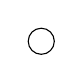
\begin{tikzpicture}[
  level distance=40 pt,
  every node/.style={circle,draw},
  level 1/.style={sibling distance=150 pt},
  level 2/.style={sibling distance=110 pt},
  level 3/.style={sibling distance=60 pt}
]
  \node {};
\end{tikzpicture}
\end{center}
\item $N(1) = 2$
\begin{center}
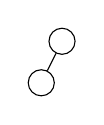
\begin{tikzpicture}[
  level distance=15 pt,
  every node/.style={circle,draw},
  level 1/.style={sibling distance=15 pt},
  level 2/.style={sibling distance=110 pt},
  level 3/.style={sibling distance=60 pt}
]
  \node {}
    child {node {}}
    child [missing];
\end{tikzpicture}
\end{center}
\item $N(2) = 4$
\begin{center}
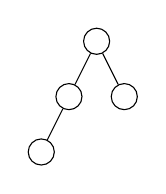
\begin{tikzpicture}[
  level distance=20 pt,
  every node/.style={circle,draw},
  level 1/.style={sibling distance=20 pt},
  level 2/.style={sibling distance=20 pt},
  level 3/.style={sibling distance=60 pt}
]
  \node {}
  	child {node {}
  		child {node {}}
  		child [missing]}
  	child {node {}};
\end{tikzpicture}
\end{center}
\end{itemize}
In general, $N(h) = 1 + N(h-1) + N(h-2)$. Observe that this sequence looks like the Fibonacci sequence: $N(h) = F_{h+3} - 1 = \displaystyle \frac{\varphi^{h+3}}{\sqrt{5}} - 1$. Doing a bit of algebra: 
\begin{align*}
N(h) &\in O(\varphi^{h+3}) \\
\log (N(h)) &\in \log(\Theta(\varphi^{h+3}) = \Theta(h)
\end{align*}
From this, we deduce that $h \in O(\log (N(h))$, and since $N(h) \leq n$, $h \in O(\log n)$.
\subsubsection{Proof of (**)}
We saw before that in a binary tree of height $h$, the number of nodes satisfies
$$n \leq 2^{h+1} - 1 \leq 2^{h+1}$$
Thus, $\log (n) \leq h+1 \iff \log(n) - 1 \leq h$, ergo $h \in \Omega(\log n)$.
\section{Dictionaries Part II}
Recall that a \textit{dictionary} is a collection of key-value pairs (KVPs). There are various ways to implement a dictionary:
\begin{itemize}
\item Unordered array or linked list
\item Ordered array
\item Balanced search trees
\end{itemize}
\subsection{Optimal Static Ordering}
Let's try to implement this dictionary through \textit{optimal static ordering}. It's referred to as `static' because this list is constructed before runtime (i.e., before a program is executed), and it's optimal because it reduces the runtime of searching for an element in the ordering.\\
The ordering involves placing the elements which are most likely to be accessed in the front of the list, this means that these elements require the least amount of time to find and they're the ones which will be searched for most often.
\subsubsection{Expected Runtime}
The expected runtime of this ordering is defined by the number of comparisons required to find any element in the ordering. The runtime depends on the respective probabilities of access for each element.\\
\begin{itemize}
\item If we have $n$ entries with a \textbf{uniform distribution} (i.e., each element has an equally likely chance of being chosen), the expected number of comparisons, $E_n$, is
$$E_n = \frac{1}{n} + 2\left(\frac{1}{n}\right) + \cdots + n\left(\frac{1}{n}\right) = \frac{n+1}{2}$$
\item If we have $n$ entries with an \textbf{exponential distribution} (i.e., the preceding element is twice as likely to be accessed then the current element), the expected number of comparisons, $E_n$, is
$$E_n = \frac{1}{2} + 2\left(\frac{1}{4}\right) + 3\left(\frac{1}{8}\right) + \cdots + (n-1)\left(\frac{1}{2^{n-1}}\right) + n\left(\frac{1}{2^{n-1}}\right)$$
Here, $E_n \in \Theta(1)$.\\
If the list was arranged in reverse as
$$\left[ \frac{1}{2^{n-1}}, \frac{1}{2^{n-1}}, \cdots, \frac{1}{4}, \frac{1}{2}\right]$$
(where the element that is \textit{least} likely to be chosen is first), then the number of comparisons, $E_n^\prime$, is
$$E_n^\prime = \left(\frac{1}{2^{n-1}}\right) + 2\left(\frac{1}{2^{n-1}}\right) + \cdots +  (n-1)\left(\frac{1}{4}\right) + n\left(\frac{1}{2}\right)$$
This runtime is $E_n^\prime \in \Theta(n)$.
\end{itemize}
\subsection{Dynamic Ordering}
What if we do not know the access probabilities ahead of time? Then we use \textbf{dynamic ordering}. This ordering involves two particular methods:
\begin{itemize}
\item \textbf{Move-To-Front (MTF):} upon a successful search, move the accessed item to the front of the list
\item \textbf{Transpose:} upon a successful search, swap the accessed item with the item immediately preceding it
\end{itemize}
This ordering mutates the list based on past search results. As the name suggests it's a dynamic approach to the optimal static ordering.
\subsection{Skip Lists}
A \textbf{skip list} is a hierarchy of ordered linked lists. For a set of $S$ items in a series of lists $S_0,S_1, \cdots, S_h$ such that:
\begin{itemize}
\item Each list $S_i$ contains the special keys $-\infty$ and $+\infty$
\item List $S_0$ contains the keys of $S$ in non-decreasing order
\item Every list contains all of the elements of every list preceding it (i.e., $S_h \subseteq S_{h-1} \subseteq \cdots S_0$)
\item $S_h$ contains only the two special keys
\end{itemize}
\begin{figure}[ht]
\begin{center}
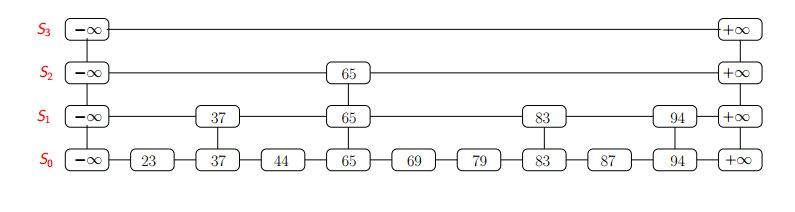
\includegraphics[scale=0.8]{skip-list.jpg}
\end{center}
\caption{An example of a skip-list. Courtesy of CS 240 lecture slides.}
\end{figure}
%END%
\end{document}